\documentclass[fontset=windows]{article}
\usepackage[margin=1in]{geometry}
\usepackage{ctex}
\usepackage{setspace}
\usepackage{lipsum}
\usepackage{graphicx}
\usepackage{caption}
\usepackage{subcaption}
\usepackage[colorlinks=true,linkcolor=red]{hyperref}
\usepackage{amsmath}
\usepackage{lmodern}

\graphicspath{{figures/}}

\title{\heiti\zihao{2} Op Amp Circuits}
\author{\songti zrrraa}
\date{2023.12.21}

\begin{document}
\maketitle
\thispagestyle{empty}

\section*{Op Amp Basics}

\begin{figure}[htbp]
    \centering
    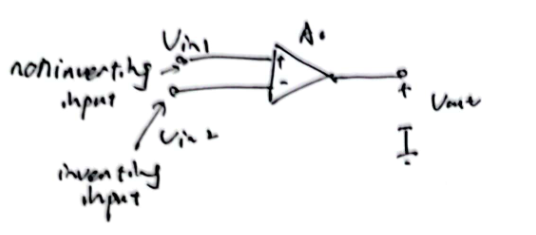
\includegraphics[scale=0.8]{1.jpg}
    \captionsetup{labelformat=empty}
    \caption{}
    \label{1}
\end{figure}

$$V_{out}=(V_{in1}-V_{in2})A_0$$

\section*{Input/Output Characteristics}

\begin{figure}[htbp]
    \centering
    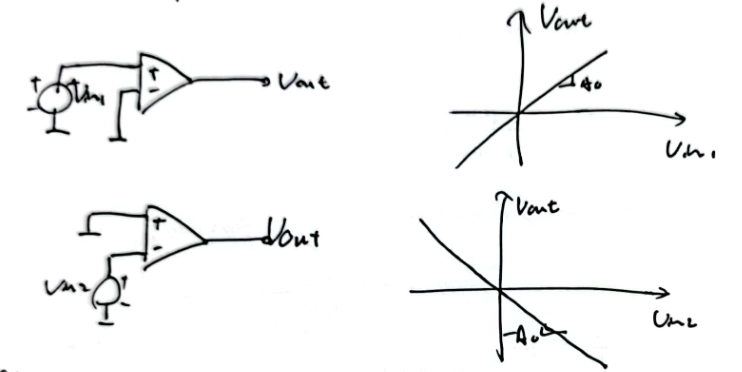
\includegraphics[scale=0.8]{2.jpg}
    \captionsetup{labelformat=empty}
    \caption{}
    \label{2}
\end{figure}

For an ideal Op Amp, Input Imp is infinite, Output Imp is zero, $A_o$ is infinite. 

\subsection*{Observations}

If $V_{out}\approx a\ few\ volts$ and $A_o\approx1000\Longrightarrow V_{in1}-V_{in2}\approx a\ few\ mV$. 

If we can visualize a complex circuit as an op amp, the analysis becomes simpler. 

\begin{figure}[htbp]
    \centering
    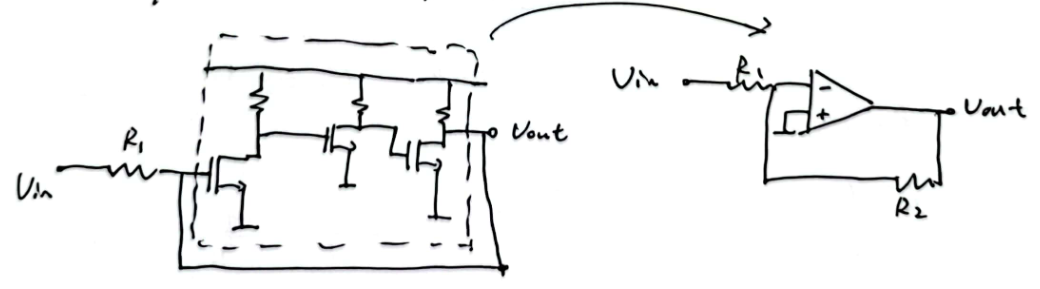
\includegraphics[scale=0.8]{3.jpg}
    \captionsetup{labelformat=empty}
    \caption{}
    \label{3}
\end{figure}

\section*{Noninverting Amplifier}

\begin{figure}[htbp]
    \centering
    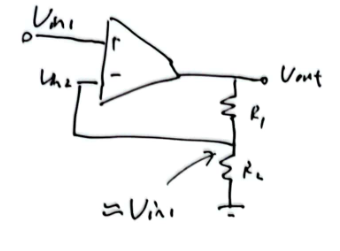
\includegraphics[scale=0.8]{4.jpg}
    \captionsetup{labelformat=empty}
    \caption{}
    \label{4}
\end{figure}

\subsection*{Case \uppercase\expandafter{\romannumeral1}: $A_o\to \infty$}

$$V_{out}=(V_{in1}-V_{in2})A_0$$

Because $A_o$ is very large and $V_{out}$ should be finite, $V_{in1}-V_{in2}$ should be very small. 

$$V_{in1}-V_{in2}\approx0\Longrightarrow V_{in1}\approx V_{in2}$$

$$\Longrightarrow V_{out}=\frac{V_{in}}{R_2}(R_1+R_2)$$

Compared with MOS amplification, using Op Amp amplification can reduce the dependence on process parameters such as transconductance, and only consider external components. 

\subsection*{Case \uppercase\expandafter{\romannumeral2}: $A_o$ is finite}

\begin{figure}[htbp]
    \centering
    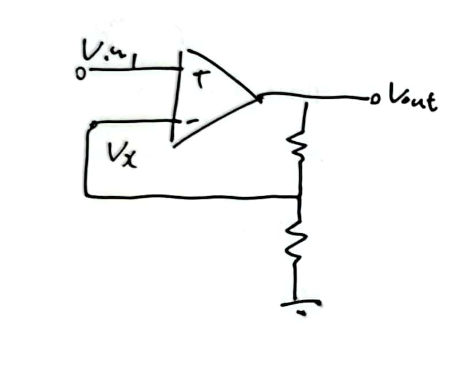
\includegraphics[scale=0.8]{5.jpg}
    \captionsetup{labelformat=empty}
    \caption{}
    \label{5}
\end{figure}

\begin{equation*}
    \begin{cases}
        V_{x}=V_{out}\frac{R_2}{R_1+R_2} \\
        (V_{in}-V_{x})A_o=V_{out}
    \end{cases}
\end{equation*}

$$\Longrightarrow \frac{V_{out}}{V_{in}}=\frac{A_o}{1+\frac{R_2}{R_1+R_2}A_o}=\frac{1}{\frac{1}{A_o}+\frac{R_2}{R_1+R_2}}$$

We call $A_o$ the open loop gain. The $\frac{V_{out}}{V_{in}}$ close loop gain. 

If $\frac{R_2}{R_1+R_2}A_o>>1\Longrightarrow \frac{V_{out}}{V_{in}}$ relatively independent of $A_o$. 

\subsection{Example}

\begin{figure}[htbp]
    \centering
    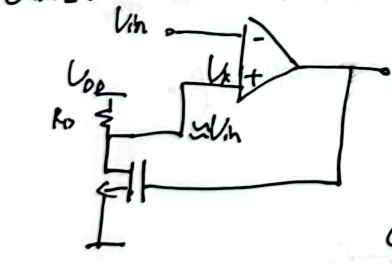
\includegraphics[scale=0.8]{6.jpg}
    \captionsetup{labelformat=empty}
    \caption{}
    \label{6}
\end{figure}

Assume $A_o\to \infty$: 

$$V_x\approx V_{in}$$

Notice that it's a CS Stage Topology:  

$$V_{out}(-g_mR_D)=V_{in}\Longrightarrow \frac{V_{out}}{V_{in}}=-\frac{1}{g_mR_D}$$

\section*{Inverting Amplifier}

\begin{figure}[htbp]
    \centering
    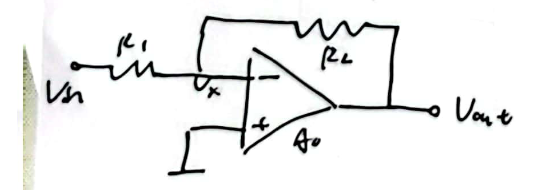
\includegraphics[scale=0.8]{7.jpg}
    \captionsetup{labelformat=empty}
    \caption{}
    \label{7}
\end{figure}

\subsection*{Case \uppercase\expandafter{\romannumeral1}: $A_o\to \infty$}

$$\frac{V_{in}}{R_1}=-\frac{V_{out}}{R_2}\Longrightarrow \frac{V_{out}}{V_{in}}=-\frac{R_2}{R_1}$$

\subsection*{Case \uppercase\expandafter{\romannumeral2}: $A_o$ is finite}

\begin{equation*}
    \begin{cases}
        V_x=\frac{V_{out}}{-A_o} \\
        \frac{V_{in}-V_x}{R1}=\frac{V_x-V_{out}}{R2}
    \end{cases}
\end{equation*}

$$\Longrightarrow \frac{V_{out}}{V_{in}}=-\frac{1}{\frac{R_1}{R_2}+\frac{1}{A_o}\frac{R_1+R_2}{R_1}}$$

Input Imp $\approx R_1$

\begin{figure}[htbp]
    \centering
    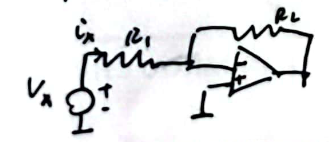
\includegraphics[scale=0.8]{8.jpg}
    \captionsetup{labelformat=empty}
    \caption{}
    \label{8}
\end{figure}

$$R=\frac{v_x}{i_x}=R_1$$

\section*{Example of Application: Voltage Regulator}

\begin{figure}[htbp]
    \centering
    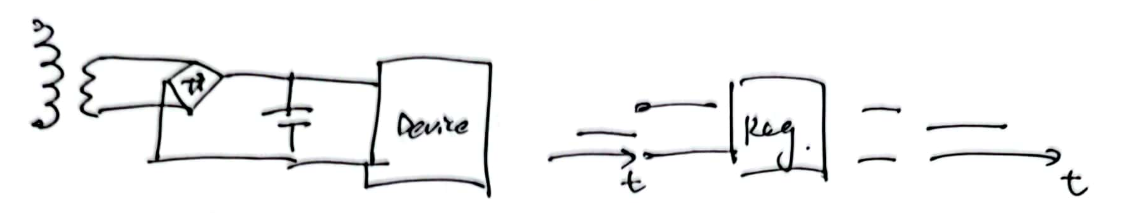
\includegraphics[scale=0.8]{9.jpg}
    \captionsetup{labelformat=empty}
    \caption{}
    \label{9}
\end{figure}

We generally need a voltage regulator in an AC-DC step-down circuit to ensure that the output voltage remains constant when the input voltage fluctuates. 

\begin{figure}[htbp]
    \centering
    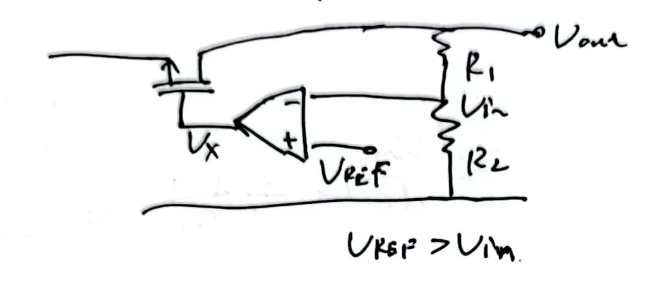
\includegraphics[scale=0.8]{10.jpg}
    \captionsetup{labelformat=empty}
    \caption{}
    \label{10}
\end{figure}

$$V_{out}\uparrow\Longrightarrow V_{in}\uparrow\Longrightarrow V_x\downarrow\Longrightarrow V_{out}\downarrow$$

Finally, $V_{out}$ will remain at a constant value. 

$$V_{out}=V_{REF}(1+\frac{R_1}{R_2})$$

\section*{Unity-Gain Buffer}

\begin{figure}[htbp]
    \centering
    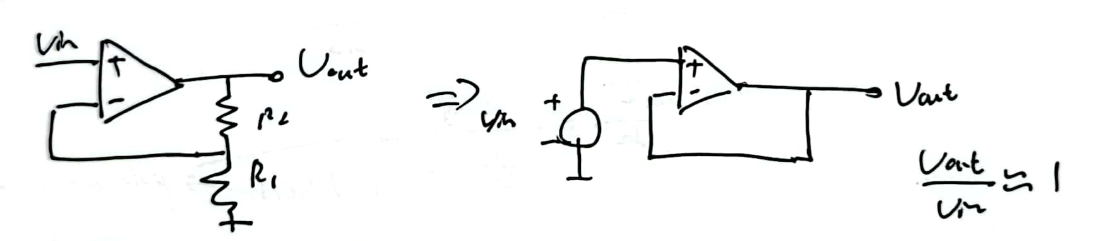
\includegraphics[scale=0.8]{11.jpg}
    \captionsetup{labelformat=empty}
    \caption{}
    \label{11}
\end{figure}

For the first topology: 

$$\frac{V_{out}}{V_{in}}\approx 1+\frac{R_2}{R_1}$$

For the second topology: 

$$\frac{V_{out}}{V_{in}}\approx 1$$

Calculate the input and output impedance below. 

Input Imp $\approx \infty \Longrightarrow$ can sense voltage without loading the circuits. 

Calculate the output impedance using Thevenin's equation. 

\begin{figure}[htbp]
    \centering
    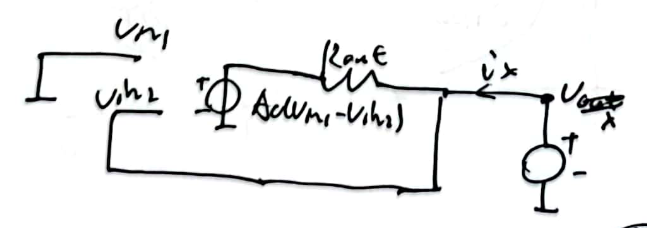
\includegraphics[scale=0.8]{12.jpg}
    \captionsetup{labelformat=empty}
    \caption{}
    \label{12}
\end{figure}

$$i_x=\frac{v_x-A_o(-v_x)}{R_{out}}$$

$$\frac{v_x}{i_x}=\frac{R_{out}}{A_o+1}$$

So we can draw like this: 

\begin{figure}[htbp]
    \centering
    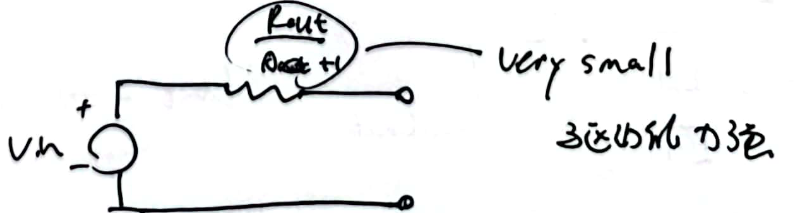
\includegraphics[scale=0.8]{13.jpg}
    \captionsetup{labelformat=empty}
    \caption{}
    \label{13}
\end{figure}

Since $A_o$ is very large, the output impedance is very small, which means that the driving capability of the circuit is very strong. 

\section*{General Inverting Amp}

\begin{figure}[htbp]
    \centering
    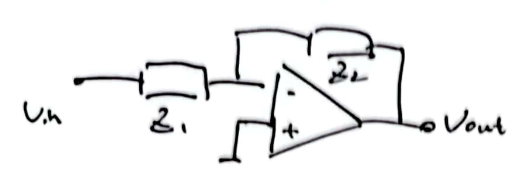
\includegraphics[scale=0.8]{14.jpg}
    \captionsetup{labelformat=empty}
    \caption{}
    \label{14}
\end{figure}

$$\frac{V_{out}}{V_{in}}\approx -\frac{Z_1}{Z_2}$$

\subsection*{Integrator}

\begin{figure}[htbp]
    \centering
    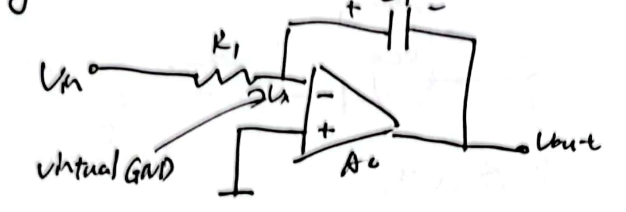
\includegraphics[scale=0.8]{15.jpg}
    \captionsetup{labelformat=empty}
    \caption{}
    \label{15}
\end{figure}

If $A_o$ is very large: 

$$\frac{V_{out}}{V_{in}}=-\frac{\frac{1}{C_1s}}{R_1}=-\frac{1}{R_1C_1s}$$

Since the pole is at the origin, the circuit gain has no bounds. 

$$\frac{-dV_{out}}{dt}C_1=\frac{V_{in}}{R_1}\Longrightarrow V_{out}=-\frac{1}{R_1C_1}\int V_{in}dt$$

If $A_o$ is finite: 

$$V_x=-\frac{V_{out}}{A_o}$$

$$\frac{V_{in}+\frac{V_{out}}{A_o}}{R_1}=\frac{-\frac{V_{out}}{A_o}-V_{out}}{\frac{1}{C_1s}}\Longrightarrow \frac{V_{out}}{V_{in}}=\frac{-1}{\frac{1}{A_o}+(1+\frac{1}{A_o})R_1C_1s}$$

Since the pole is not the origin, the circuit gain has a bound. 

\subsection*{Differentiator}

\begin{figure}[htbp]
    \centering
    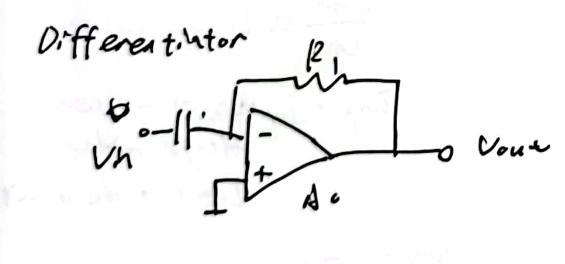
\includegraphics[scale=0.8]{16.jpg}
    \captionsetup{labelformat=empty}
    \caption{}
    \label{16}
\end{figure}

$$\frac{V_{out}}{V_{in}}=-\frac{R_1}{\frac{1}{C_1s}}=-R_1C_1s$$

Plot the frequency response: 

\begin{figure}[htbp]
    \centering
    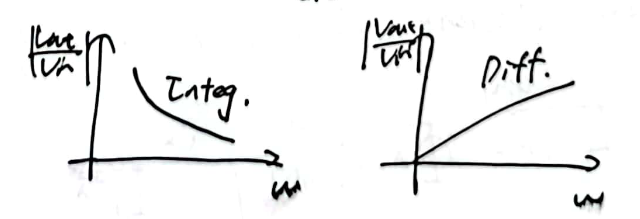
\includegraphics[scale=0.8]{17.jpg}
    \captionsetup{labelformat=empty}
    \caption{}
    \label{17}
\end{figure}

\section*{Voltage Adder (Summer)}

\begin{figure}[htbp]
    \centering
    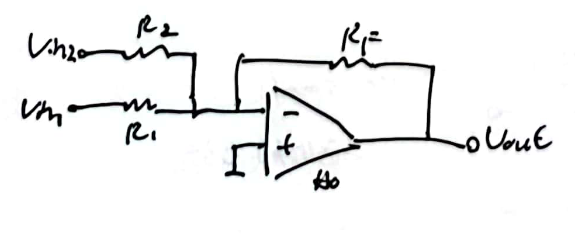
\includegraphics[scale=0.8]{18.jpg}
    \captionsetup{labelformat=empty}
    \caption{}
    \label{18}
\end{figure}

$$V_{out}=-R_F(\frac{V_{in1}}{R_1}+\frac{V_{in2}}{R_2})$$

\section*{Link}

\href{https://www.bilibili.com/video/BV1FD4y1R7Ah?p=42&vd_source=1d0c07486a3bd3b0adb8ac548bf6453e}{Razavi Electronics Circuits 1: lectrue 42}

\href{https://www.bilibili.com/video/BV1FD4y1R7Ah?p=43&vd_source=1d0c07486a3bd3b0adb8ac548bf6453e}{Razavi Electronics Circuits 1: lectrue 43}
\end{document}